
\section{Application to Cryptographic Primitives}
\label{sec:p_encodings_implementations}


In this section, we apply our approach on some cryptographic primitives. For each primitive, we first explain the construction of the gadgets required and report the concrete performances of our implementation. We detailed all the timings of our experimentations along with the sets of parameters we used in Section \ref{sec:tables_perfs}.

For performance measurement, we implemented our framework in our fork of the library \texttt{tfhe-rs} \cite{tfhe-rs} adapted as discussed in Section \ref{sec:p_encodings_TFHE_adaptation} and we generated the sets of parameters thank to our version of \texttt{concrete-optimizer} \cite{concrete-optimizer}. By default, we tailored the sets of parameters to limit the probability of failure $\epsilon$ of a bootstrapping to $2^{-40}$, and a security level of $\lambda = 128$ bits. All experiments have been carried out on a laptop with a 12th Gen Intel(R) Core(TM) i5-1245U CPU with 10 cores and a frequency of 4.4 GHz, and 16 GB of RAM.


\subsection{SIMON Block Cipher}
\label{sec:simon}

SIMON is a hardware-oriented block cipher developed in \cite{simon}, which relies only on the following operations: \texttt{AND}, rotation, \texttt{XOR}. It is a classical Feistel network for which the Feistel function consists in applying basic operations on the branch, xoring the subkey and then xoring the result with the other branch as depicted in the Figure~\ref{fig:simon_cipher} (on this figure, $S^i$ denotes the left circular shift by $i$ bits.). We use one ciphertext per bit so the rotation operation is essentially free. Note that the key is considered as a plaintext, which does not change anything in the framework. In our implementation, we considered a (128-128) instance of SIMON (i.e. the whole state and the key are of size 128). 


% \begin{wrapfigure}{r}{5.5cm}
% 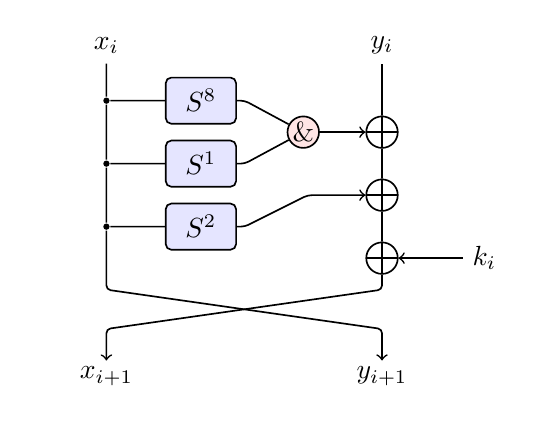
\begin{tikzpicture}
  [line width=0.6,trim left,
   shiftbox/.style = {
     draw, fill=blue!10, rounded corners=2pt,
     inner xsep=0.25cm, inner ysep=0.15cm,
   },
   wire/.style = {
     rounded corners=1.5pt
   },
   xor/.style = {
     draw, circle, inner sep=0cm, minimum size=0.4cm,
     append after command = {
       [shorten >=\pgflinewidth, shorten <=\pgflinewidth,]
       (\tikzlastnode.north) edge (\tikzlastnode.south)
       (\tikzlastnode.east) edge (\tikzlastnode.west)
     }
   },
   odot/.style = {
     draw, circle, inner sep=0cm, minimum size=0.4cm,fill=red!10
   },
   dot/.style = {
     fill, circle, inner sep=0cm, minimum size=0.08cm
   }]

  %Draw nodes
  \node at (1,6.7) (xin) {$x_i$};
  \node at (4.5,6.7) (yin) {$y_i$};
  \node[dot] at (1,6) (d1) {};
  \node[dot] at (1,5.2) (d2) {};
  \node[dot] at (1,4.4) (d3) {};
  \node[shiftbox] at (2.2,6) (S1) {$S^8$};
  \node[shiftbox] at (2.2,5.2) (S2) {$S^1$};
  \node[shiftbox] at (2.2,4.4) (S3) {$S^2$};
  \node[xor] at (4.5,5.6) (x1) {};
  \node[xor] at (4.5,4.8) (x2) {};
  \node[xor] at (4.5,4.0) (x3) {};
  \node[odot] at (3.5,5.6) (AND) {\&};
  \node at (5.8,4.0) (k) {$k_i$};
  \node at (1, 2.5) () {$x_{i+1}$};
  \node at (4.5, 2.5) () {$y_{i+1}$};

  %Draw wires
  \draw[wire] (d1) -- (S1)  (S1.east) -- +(0.1,0) -- (AND);
  \draw[wire] (d2) -- (S2)  (S2.east) -- +(0.1,0) -- (AND);
  \draw[wire,->] (AND) -- (x1);
  \draw[wire,->] (d3) -- (S3) (S3.east) -- +(0.1,0) -- ++(0.9,0.4) -- (x2);
  \draw[wire,->] (xin) -- (d1) -- (d2) -- (d3)
                  -- ++(0,-0.8) -- ++(3.5,-0.5) -- ++(0,-0.4);
  \draw[wire,->] (yin) -- (x1) -- (x2) -- (x3)
                 -- ++(0,-0.4) -- ++(-3.5,-0.5) -- ++(0,-0.4);
  \draw[wire,->] (k.west) -- (x3);
\end{tikzpicture} 
%    \caption{One Feistel round of SIMON. }   
%    \label{fig:simon_cipher}
% \end{wrapfigure}

\begin{figure}
    \centering
    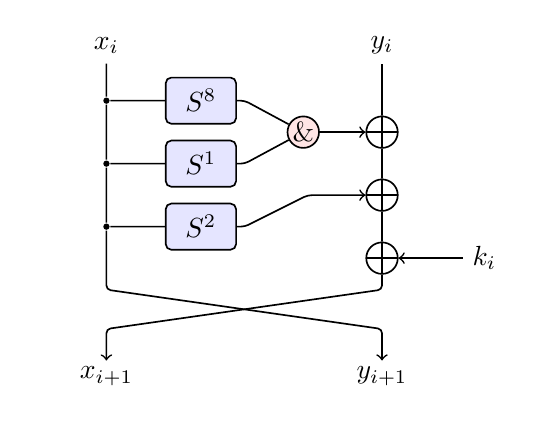
\begin{tikzpicture}
  [line width=0.6,trim left,
   shiftbox/.style = {
     draw, fill=blue!10, rounded corners=2pt,
     inner xsep=0.25cm, inner ysep=0.15cm,
   },
   wire/.style = {
     rounded corners=1.5pt
   },
   xor/.style = {
     draw, circle, inner sep=0cm, minimum size=0.4cm,
     append after command = {
       [shorten >=\pgflinewidth, shorten <=\pgflinewidth,]
       (\tikzlastnode.north) edge (\tikzlastnode.south)
       (\tikzlastnode.east) edge (\tikzlastnode.west)
     }
   },
   odot/.style = {
     draw, circle, inner sep=0cm, minimum size=0.4cm,fill=red!10
   },
   dot/.style = {
     fill, circle, inner sep=0cm, minimum size=0.08cm
   }]

  %Draw nodes
  \node at (1,6.7) (xin) {$x_i$};
  \node at (4.5,6.7) (yin) {$y_i$};
  \node[dot] at (1,6) (d1) {};
  \node[dot] at (1,5.2) (d2) {};
  \node[dot] at (1,4.4) (d3) {};
  \node[shiftbox] at (2.2,6) (S1) {$S^8$};
  \node[shiftbox] at (2.2,5.2) (S2) {$S^1$};
  \node[shiftbox] at (2.2,4.4) (S3) {$S^2$};
  \node[xor] at (4.5,5.6) (x1) {};
  \node[xor] at (4.5,4.8) (x2) {};
  \node[xor] at (4.5,4.0) (x3) {};
  \node[odot] at (3.5,5.6) (AND) {\&};
  \node at (5.8,4.0) (k) {$k_i$};
  \node at (1, 2.5) () {$x_{i+1}$};
  \node at (4.5, 2.5) () {$y_{i+1}$};

  %Draw wires
  \draw[wire] (d1) -- (S1)  (S1.east) -- +(0.1,0) -- (AND);
  \draw[wire] (d2) -- (S2)  (S2.east) -- +(0.1,0) -- (AND);
  \draw[wire,->] (AND) -- (x1);
  \draw[wire,->] (d3) -- (S3) (S3.east) -- +(0.1,0) -- ++(0.9,0.4) -- (x2);
  \draw[wire,->] (xin) -- (d1) -- (d2) -- (d3)
                  -- ++(0,-0.8) -- ++(3.5,-0.5) -- ++(0,-0.4);
  \draw[wire,->] (yin) -- (x1) -- (x2) -- (x3)
                 -- ++(0,-0.4) -- ++(-3.5,-0.5) -- ++(0,-0.4);
  \draw[wire,->] (k.west) -- (x3);
\end{tikzpicture} 
    \caption{One Feistel round of SIMON. }     
    \label{fig:simon_cipher}
\end{figure}


The Boolean function to evaluate can be defined as $$f(b_0, b_1, b_2, b_3, b_4) = b_0 \cdot b_1 \oplus b_2 \oplus b_3 \oplus b_4~.$$


Using Algorithm \ref{alg:add_element}, we found the smallest possible $p$ ($p = 9$) and the following $9$-encodings to evaluate each bit of the Feistel function with one single bootstrapping (i.e. totalling 64 PBS per round). 


\[\Encoding_0 = \Encoding_1 = \EncDefOne{1} \text{ and } \Encoding_2 = \Encoding_3 = \Encoding_4 = \EncDefOne{2} \text{ with } p = 9.\] The sum of these $p$-encodings yields the output encoding: \[\Encoding_{out} = \EncDef{\{0, 1, 4, 5, 8\}}{\{2, 3, 6, 7\}} \text{ with } p=9\] which is valid for $f$. After the PBS, all the bits of the state are encrypted under the encoding $\Encoding_0$. We formalize that with the gadget $\Gamma = \left ((\Encoding_0, \Encoding_1, \Encoding_2, \Encoding_3, \Encoding_4), \Encoding_0, 9, 9\right )$


To perform a Feistel round on a state of size $k$, the gadget $\Gamma$ is applied in parallel $k / 2$ times. Note that one bit may be used in several evaluation as $b_0$, $b_1$ and $b_2$. So we sometimes have to switch from $\Encoding_0$ to $\Encoding_1$ by a simple external multiplication by $2$, which is negligible in terms of performances.


Using our version of \texttt{concrete-optimizer} \cite{concrete-optimizer}, we crafted a set of parameters suitable for this modulus and these encodings. 
On our machine, one PBS with such parameters takes about $9.5$ ms. The theoretical timings achieved on one full block without any parallelization is $41$ seconds ($68$ rounds $\times$ $64$ bits $\times$ $9.5$ ms)  which we confirmed experimentally.


Nonetheless, this setting is intrinsically parallelizable: the 64 gadgets of each round can be performed in parallel. We implemented parallelization using the module \texttt{Rayon} of Rust, which made the total timings drop to $13$ seconds on our machine. 

Compared to \cite{DBLP:conf/fps/BendoukhaSSQS22} that implemented the same block cipher on an equivalent hardware with parallelism, our implementation is about 10 times faster. Table \ref{tab:concrete_perfs} shows the comparison. Note that in this paper, the probability of failure is not specified. As ours is pretty conservative, this is a good argument in favor of our framework.


\subsection{The Trivium Stream Cipher}
\label{sec:trivium}

Trivium \cite{ISC:DeCanniere06} is a stream cipher that uses a circular state. At each round, the bits are rotated within the state, except for three of them that are refreshed using the Boolean function of Section \ref{sec:simon}. The outer stream is generated by xoring three bits of the state each round once a ``warming-up'' phase is achieved. 


For each generated key bit, it requires performing this function three times and aggregating five \texttt{XOR} operations in the center. Our strategy is to evaluate the refreshing function three times per round with one PBS for each of them, then get the result in $\Z_2$ and chain the five \texttt{XOR} operations to get the output.
Figure \ref{fig:triviuml} illustrates the layout of the cipher.
\begin{figure}
    \centering
    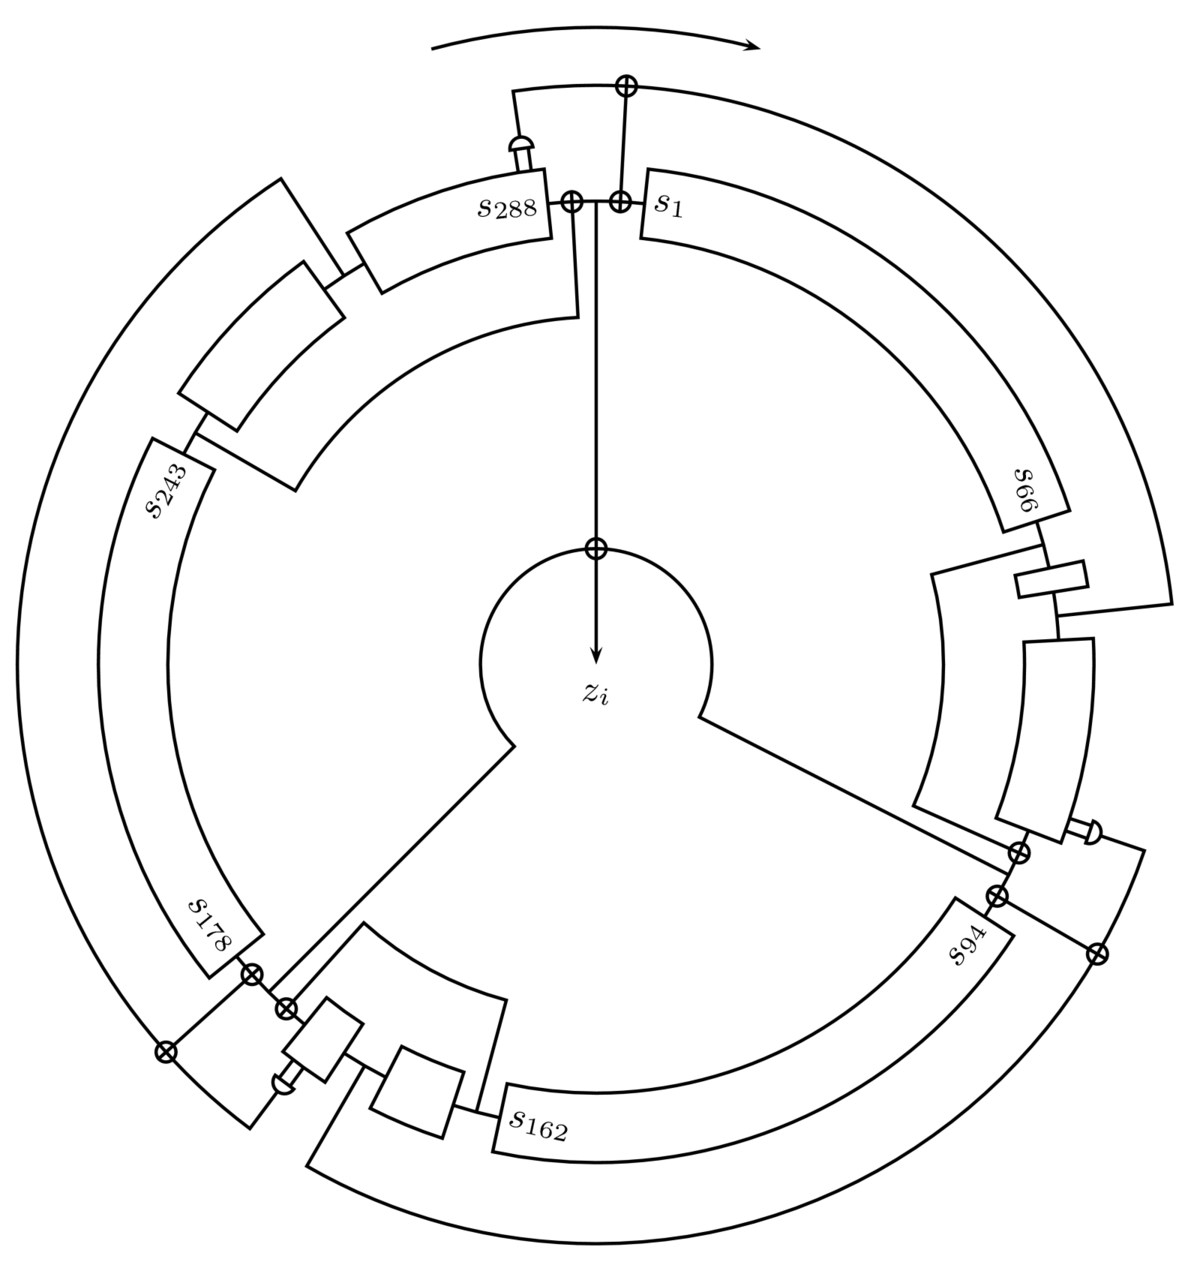
\includegraphics[width=0.5\linewidth]{img/to_harmonize/trivium.png}
    \caption{The trivium stream cipher. Figure extracted from \cite{ISC:DeCanniere06}}.
    \label{fig:triviuml}
\end{figure}


In \cite{DBLP:conf/wahc/BalenboisOS23}, the authors implement Trivium using the original \texttt{tfhe-rs} library, with 2 bits of message and 2 bits of carry for a total of 4 significative bits out of the 32 of a ciphertext component. They call this mode the \texttt{shortint} mode. The use-case they target is transciphering.

To compare our implementation with the one of \cite{DBLP:conf/wahc/BalenboisOS23}, timings are not a good metric as in their work they are provided on a massive AWS instance with a significant amount of parallelism. A better metric is to count the number of PBS and compare the parameter sets.

We reproduced the PBS operation with their parameter set on our machine and then simply estimated the timings of one round of Trivium with their approach with no parallelism. The results are summed up in Table \ref{tab:perfs_trivium}. Note that in our implementation we do not refresh the output bits with a PBS after the chain of \texttt{XOR}, because in the use-case of transciphering one more \texttt{XOR} has to be performed with the message. We take advantage of this and move the last PBS into the transciphering phase.

\begin{table}[htbp]
\centering
\caption{Comparison of timings of one round of Trivium between our work and \cite{DBLP:conf/wahc/BalenboisOS23}, with $\epsilon=2^{-40}$.}
\label{tab:perfs_trivium}
\begin{tabular}{|c|c|c|c|}
\hline
Instance & Timing PBS & Number of PBS per round & Estimated timings \\
\hline
\cite{DBLP:conf/wahc/BalenboisOS23} & 6.6 & 7 & 46.2 ms \\
\hline
Our work & 9.5 & 3 & 28.5 ms \\
\hline
\end{tabular}
\end{table}

\subsection{Keccak Permutation}
\label{sec:keccak}

Keccak is a hash function standardized by NIST under the name \emph{SHA-3} \cite{sha-3}. It is a sponge function, whose transformation is called the \emph{Keccak permutation}. It consists of five sub-functions: $\theta$, $\rho$, $\pi$, $\chi$, and $\iota$.

Let us recall that our approach encrypts each bit in one TFHE ciphertext. Let us explain the stategies of homomorphization of these sub-functions:
\begin{itemize}
    \item $\rho$ and $\pi$ simply reorder the bits within the state, so they are not impacted by the homomorphization.
    \item $\theta$ is just a serie of \texttt{XOR} operations, so it can be performed with a serie of homomorphic additions and without any PBS provided that the input ciphertexts are defined over $\Z_p$ with $p=2$.
    \item $\chi$ is the only non-linear function of the permutation, and has to be performed with a PBS. It is the transformation that applies the function defined by $$f_\chi(a, b, c) = a \oplus c \oplus b \& c$$ to get each bit of the output state.
    \item Finally, $\iota$ performs a simple \texttt{xor} with a constant, so it can be handled in a similar manner that $\theta$. The difference is that the constant is in clear this time.
\end{itemize}
The $p$-encodings we use are:
\begin{itemize}
    \item $\Encoding_{\&} = \EncDef{\{1\}}{\{2\}}$ with $p_\& = 3$  to evaluate the $\&$ operator in the alternative formula of $\chi$.
    \item $\Encoding_\oplus = \EncDefOne{1}$ with $p_\oplus = 2$ for the other operations of $\oplus$.
\end{itemize}
Our strategy of homomorphic evaluation of the Keccak permutation is as follows:
\begin{enumerate}
    \item Encrypt the input state under the encoding $\Encoding_\oplus$.
    \item Evaluate the subfuctions $\theta$, $\rho$, and $\pi$. Theses functions being purely linear, they can be performed only with sums under $\Encoding_\oplus$.
    \item Change the encoding from $\Encoding_\oplus$ to $\Encoding_\&$ with one PBS per bit of the state (Property \ref{prop:enc_switch_pbs}).
    \item Evaluate the \texttt{AND} operator of the subfunction $\chi$ with the gadget \[\Gamma_\& = \left ( (\Encoding_\&, \Encoding_\&), \Encoding_\oplus, 3, 2\right )\] associated to function $f_\& : (x, y) \mapsto x \& y$. This gadget is applied once per bit of the state.
    \item Evaluate the remaining $\oplus$ operators of $\chi$ and the $\iota$ subfunctions, then jump back Step 2. for the next loop iteration.
\end{enumerate}


Casting a ciphertext from $\Encoding_\oplus$ to $\Encoding_\&$ (Step 3) is a bit tricky because $p_\oplus = 2$ is even. Because of the negacyclicity problem, one needs $\Encoding_\&(0) = \modulo{-\Encoding_\&(1)}{p_\&}$. With $p_\& = 3$, the only candidate is the encoding $\Encoding_\&$ defined above.


As a result, each round takes two programmable bootstrappings per bit. An implementation with our tweaked version of \texttt{tfhe-rs} takes 16.5 seconds (without any parallelism) on our hardware to perform one Keccak round on a state of 1600 bits in spite of the two PBS required per round and per bit. Those timings are possible because of the small values of $p$ allowing the use of a set of  small parameters, which speeds up the computation. A full run of Keccak counting 24 rounds, we can then estimate the timings without parallelism to $6.6$ minutes. For the sake of simplicity, we use the same set of parameters for both types of PBS, avoiding the hassle of using two different server keys.


This strategy of implementation complies with the more generic one that we introduce in Section \ref{sec:ascon} and that is illustrated on Figure \ref{fig:layout_spn}. It suits very well the use-cases where linear and non-linear operations are alternating.


\subsection{Ascon}
\label{sec:ascon}


Ascon \cite{JC:DEMS21, asconv12nist} is a lightweight block cipher algorithm that was designed to provide efficient and secure encryption and authentication for a wide range of applications, particularly in resource-constrained environments such as embedded systems and IoT devices. The name ``Ascon'' stands for ``Authenticated encryption for Small Constrained Devices''. We implemented its s-box, whose circuit is represented on Figure \ref{fig:ascon}.

\begin{figure}[h]
    \centering
    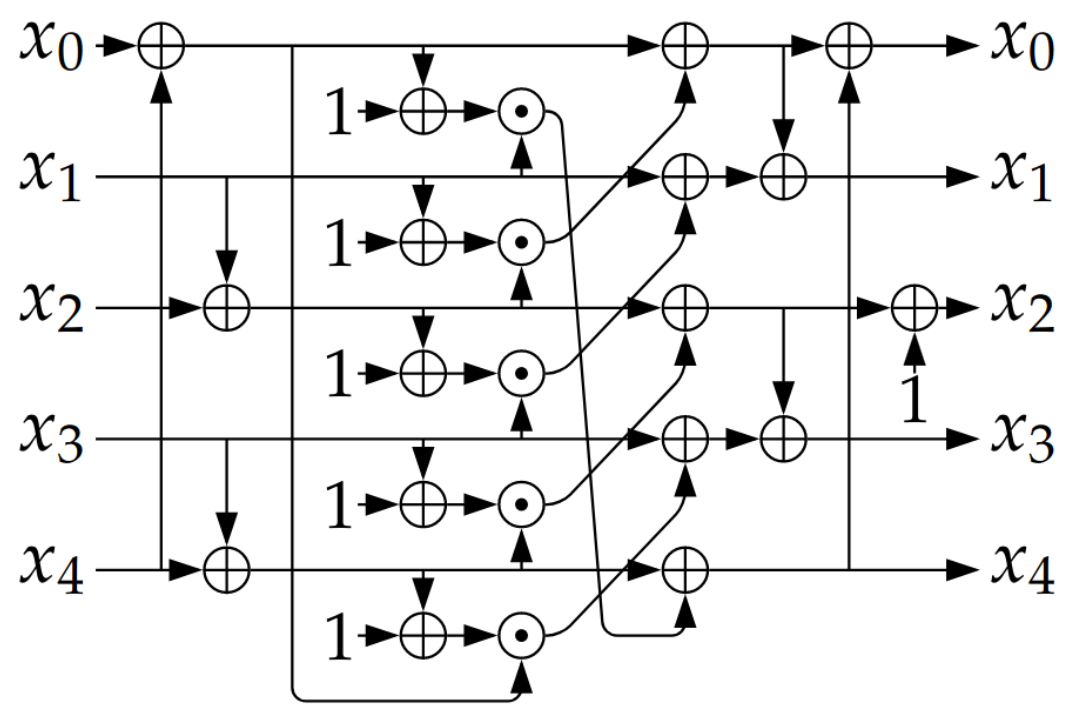
\includegraphics[width=0.5\linewidth]{img/to_harmonize/ascon.png}
    \caption{The 5-bits look-up table of ASCON. Figure extracted from \cite{JC:DEMS21}}
    \label{fig:ascon}
\end{figure}



This layout is a bit different from the others: the s-box takes five bits as input and outputs five bits. We denote $f_0, \dots, f_4$ the five functions of $\B^5 \mapsto \B$ that generate the 5 output bits $x_0, \dots, x_4$. Thus, we need to define five gadgets (one per function).

These functions, once analyzed by the algorithm, can be computed in one single bootstrapping each, but for different values of $p$ (respectively $p=17, 7, 7, 15, 11$ that are the smallest possible values). We could implement the gadgets $\Gamma_0, \dots, \Gamma_4$ (associated to $f_0, \dots, f_4$) with different values for $p_{in}$, but this would imply to introduce some encoding switchings before each round of hashing. To keep things simpler we generated only encodings with $p = 17$, making the implementation more straightforward as no encoding switching is required. For each subfunction $f_i$, five canonical $17$-encodings $(\Encoding_{i, 0}, \dots, \Encoding_{i, 4})$ of form $$\Encoding_{i, j} = \EncDefOne{d_{i,j}}$$ are computed. The results are displayed in the Table \ref{tab:encodings_ascon}. Note the zero values in some cases, they show that the variable is not used in the subfunction. 

The s-box layer is followed by a linear layer, where the bits of the states are shifted and combined with \texttt{XOR} operations. This can be trivially done with $p=2$. Finally, to prepare the next round, an encoding switching is performed to send back the ciphertexts on $17$-encodings. This is summed up in Figure \ref{fig:layout_spn}. Note that there is no encoding switching from non-linear layer to linear layer because the gadgets can directly outputs ciphertexts under $\Encoding_\oplus = \EncDefOne{1}$ with $p=2$.

\begin{figure}
    \centering
    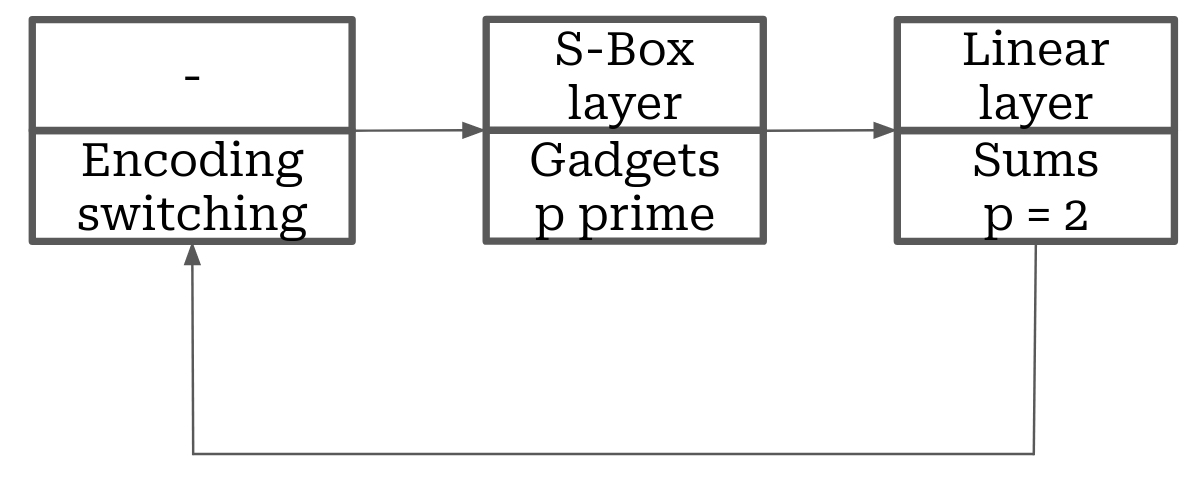
\includegraphics[width=0.5\linewidth]{img/to_harmonize/layout_spn.png}
    \caption{A common layout to evaluate cryptographic primitives. The upper part of the boxes represents what happens in the clear, while the lower part shows the encrypted operations. }
    \label{fig:layout_spn}
\end{figure}


To wrap up, we construct the five gadgets $\Gamma_i = \left ( (\Encoding_{i,0}, \dots,  \Encoding_{i, 4}), \Encoding_\oplus, 17, 2, f_i \right )$. They will carry the evaluation of the s-boxes and output ciphertexts encrypted under $\Encoding_\oplus$. Then, the linear layer is trivially evaluated with homomorphic sums. An encoding switching from $\Encoding_\oplus$ to $\Encoding_{i, j}$ allows to come back to non-linear operations.




\begin{table}[]
    \centering
    \begin{tabular}{|c|c|c|c|c|c|}
        \hline
       subfunction & $d_{i, 0}$ & $d_{i, 1}$ & $d_{i, 2}$ & $d_{i, 3}$ & $d_{i, 4}$\\
        \hline
        $f_0$  & $1$ & $2$ & $3$ & $7$ & $14$\\
        \hline
        $f_1$ & $1$ & $2$ & $2$ & $2$ & $4$\\
        \hline
        $f_2$ & $1$ & $2$ & $2$ & $4$ & $0$\\
        \hline
        $f_3$ & $1$ & $1$ & $5$ & $5$ & $3$\\
        \hline
        $f_4$ & $1$ & $2$ & $0$ & $4$ & $3$\\
        \hline
     \end{tabular}
    \caption{Parameters $d_{i, j}$ for Ascon, with $p=17$ for every subfunction.}
    \label{tab:encodings_ascon}
\end{table}


Using this solution, the s-box is evaluated in $92$ ms. Note that the 5 different PBS described in Table \ref{tab:encodings_ascon} have different norms of vector $\vec d$ so they may have a different set of parameters for each. We use the more restrictive one (i.e. the one with greater $\norm{\nu}$) for the 5. Estimating the timings of a full run of Ascon is not trivial because it depends a lot of the parameters. To give a rough idea, in hashing mode, 64 s-boxes are required per round, with 12 rounds recommended. The outputs of the s-boxes are in $\Z_2$ to allow the evaluation of the linear layer of Ascon. At the end of this linear layer, the encoding of each of the 320 bits of the state must be switched back to $\Z_{17}$ with a PBS. To do so, we use the same set of parameters as for the encoding switching in Step 3 of the Keccak evaluation in Section \ref{sec:keccak}.

This gives an estimation of $89$ seconds for one Ascon hash.

